\begin{figure*}[hbt!]
\centering
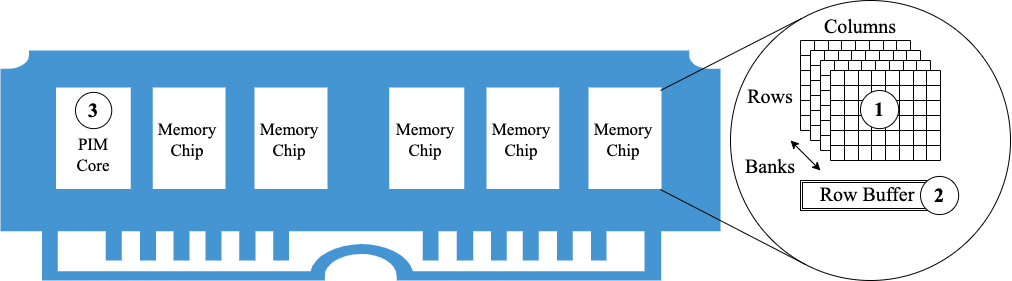
\includegraphics[width=.8\linewidth]{MEMSYS22/figures/pimcat.png}
%\vspace{.5em} 
\caption{Generic representation of a Main Memory DIMM. Processing in memory can take place at the (1) memory array, (2) row buffer or in a simple processing unit (3) closer to the banks}.
%\vspace{-1.5em} 
\label{fig:pimcat}
%\vspace{-0.6cm}    
\end{figure*}   
%\looseness -1




Processing in memory generally refers to the idea of moving some of the executions to the memory unit, when moving the data to the CPU for processing deem to take more time, which is often the case for memory intensive kernels. With various memory technologies and PIM optimization techniques present, there are several ways PIM can be adopted. Figure~\ref{fig:pimcat} shows a generic representation of a main memory DIMM module. A main memory DIMM (e.g. DDR4 DIMM) has several chips. Each chip has a number of banks (e.g. 4, 8, 16) and each bank has a specified number of rows and columns which constitutes the memory array (highlighted as \circled{1} in Figure ~\ref{fig:pimcat}). Each intersection of a row and column typically represents a memory \textit{cell} which holds single bit data. When a row address is requested to be accessed, that selected row is then loaded on to the row buffer (highlighted as \circled{2} in Figure ~\ref{fig:pimcat}). 

Several studies propose to use the memory array \circled{1} for computing \cite{03,06,13,15,20,29}, mostly for matrix vector multiplication operations where the coefficients can be mapped to the rows and columns to compute dot products using the array. Baohua et al. \cite{13} propose to improve in-memory multiplication with partition-based computation techniques for broadcasting and moving data within partitions. The authors exploit ReRAM's voltage controlled variable resistance to support logic gates. Long et al. \cite{20} proposes another ReRAM based design particularly for Recurrent Neural Network (RNN) acceleration. The study proposes crossbar sub-arrays for matrix vector multiplication, multiplier sub-arrays for element-wise operations and special function units for nonlinear functions. Peng et al. \cite{15} present a new mapping method and data flow to maximize reuse of weight and input data on a 8-bit ReRAM based PIM architecture. Imani et al. \cite{6} report to have achieved graph processing and query processing capabilities along with machine learning acceleration with processing in memory.  


%Since applications from these domains frequently use matrix vector multiplication operations, where the coefficients can be naturally mapped to the word-lines (WL) and bit-lines (BL) and use the data array to compute the dot product in the each cell then eventually accumulating them along the source-lines (SL) \cite{15,20}.

The second category of PIM operations are proposed in the row buffer level \circled{2}; for example, by adding multiple row buffers and performing bit-wise operations among them. Lin et al. \cite{31} present PIM design proposing optimization at the row buffer level. The authors introduce a \textit{Population Count Engine} which works on the data inside the sense amplifier and store the results back to the sense amplifier.

The third category of processing in memory suggests to have a simple processing unit near the memory banks (marked as \circled{3} in Figure~\ref{fig:pimcat}) capable of executing a sub-set of CPU instructions. The main intention of this model is to reduce memory traffic to/from CPU \cite{01,02,05,11,12,17,30,32,33,34,35,71}. Some of these studies suggest to use the logic die of 3D stacked memories to place Processing Elements (PE) directly beneath the DRAM dies with shorter distance to the coefficient data residing in the DRAM layers for faster computation \cite{09,12,30,32}.  Huang et al. \cite{33} propose a heterogeneous PIM design incorporating memristors and CMOS based technologies, in order to accommodate the heterogeneity requirements of graph applications. DAMOV~\cite{71} is a PIM simulation infrastructure based on ZSim\fixme{[]} and Ramulator \fixme{[]} with offloading support. The authors develop a rigorous workload characterization methodology and quantify data movement bottleneck on an extensive set of applications and functions. Few studies evaluate PIM architectures with hardware implementation. Lee et al. \cite{12} develops an industrial prototype of a PIM design that can seamlessly work with a variety of commercial processors without requiring any changes on the applications. The proposed PIM execution unit has a five-stage pipeline, 16-wide SIMD FPU, registers and controller. This design is based on a HBM stack which is fabricated with a 20nm technology process. PimCaffe \cite{16} develops a PIM near memory design based on multiple FPGAs, implementing SIMD and systolic array compute engines for vector and matrix multiplications.    

As a general observation, first two approaches of PIM design (processing in memory array and row buffer) are inherently limited to certain compute operations. Since HPC application kernels perform complex computations that frequently includes floating point operations with various arithmetic functions, we believe the PIM execution model that would serve the best for HPC domain is the third approach explained above --- to employ a simple processing unit where memory intensive HPC kernels can be offloaded in its entirety to be executed. In this work, we evaluate HPC kernels on a simple processing unit closer to the memory as detailed in Section~4. 

% and the majority of the studies exploring this category attempts to accelerate application segments from Machine Learning, AI and Neural Network domain .  

%+++++++++++++++++++++++++++++++++++++++++++++++++++++++++++++=

%Several recent studies explore the architectural scope and application domains of processing in memory.

%\subsection{Architectural Scope of PIM}

%Processing in the memory array is addressed in several studies~\cite{03,06,13,15,20,29}. Leitersdorf et al. 


%Majority of the studies adopt near memory compute unit equipped with simple core(s) \cite{01,02,05,11,12,17,30,32,33,34,35}.        

%\subsection{Application Domain}

%The vast majority of the studies  \cite{03,04,08,09,10,11,14,15,16,18,19,20,22,29,31}.     









%-	PIM background \\
%-	Different types of PIM \\
%\textbf{-	Which type of PIM can be beneficial for HPC and why?} \\




  